\documentclass[12pt,a4paper]{report}

% --- Encodage ---
\usepackage[utf8]{inputenc}
\usepackage[T1]{fontenc}

% --- Mise en page ---
\usepackage[top=2.5cm,bottom=2.5cm,left=3cm,right=2.5cm]{geometry}
\usepackage{setspace}
\setstretch{1.3}

% --- Couleurs ---
\usepackage{xcolor}
\definecolor{PrimaryBlue}{RGB}{15,70,145}
\definecolor{AccentGold}{RGB}{200,155,30}
\definecolor{LightBlue}{RGB}{230,240,255}
\definecolor{LightGold}{RGB}{255,250,230}
\definecolor{LightGreen}{RGB}{230,250,235}
\definecolor{LightRed}{RGB}{255,235,235}
\definecolor{CodeBg}{RGB}{248,248,252}
\definecolor{CodeFrame}{RGB}{195,205,225}
\definecolor{KwColor}{RGB}{0,0,190}
\definecolor{CmtColor}{RGB}{40,130,40}
\definecolor{StrColor}{RGB}{160,0,0}
\definecolor{GrayText}{RGB}{100,100,110}
\definecolor{DarkGray}{RGB}{50,50,60}

% --- Code ---
\usepackage{listings}
\usepackage{lstautogobble}
\lstdefinestyle{cppstyle}{
  language=C++,
  backgroundcolor=\color{CodeBg},
  frame=single, rulecolor=\color{CodeFrame},
  basicstyle=\ttfamily\footnotesize,
  keywordstyle=\color{KwColor}\bfseries,
  commentstyle=\color{CmtColor}\itshape,
  stringstyle=\color{StrColor},
  numberstyle=\tiny\color{GrayText},
  numbers=left, numbersep=8pt,
  tabsize=4, breaklines=true,
  keepspaces=true, showstringspaces=false,
  autogobble=true,
  morekeywords={uint32_t,uint8_t,double,float,bool,nullptr,
                constexpr,inline,auto,struct,static_assert},
}
\lstset{style=cppstyle}

% --- Maths ---
\usepackage{amsmath,amssymb}

% --- Tableaux ---
\usepackage{booktabs,tabularx,array}
\newcolumntype{C}[1]{>{\centering\arraybackslash}p{#1}}

% --- Boites colorees ---
\usepackage{tcolorbox}
\tcbuselibrary{skins,breakable,theorems}

\newtcolorbox{conceptbox}[1][Concept]{
  colback=LightBlue, colframe=PrimaryBlue, coltitle=white,
  fonttitle=\bfseries\small, title={#1},
  boxrule=0.8pt, arc=5pt, breakable,
  left=6pt, right=6pt, top=5pt, bottom=5pt}

\newtcolorbox{resultbox}[1][Resultats]{
  colback=LightGreen, colframe=green!50!black, coltitle=white,
  fonttitle=\bfseries\small, title={#1},
  boxrule=0.8pt, arc=5pt,
  left=6pt, right=6pt, top=5pt, bottom=5pt}

\newtcolorbox{warnbox}[1][Attention]{
  colback=LightRed, colframe=red!60!black, coltitle=white,
  fonttitle=\bfseries\small, title={#1},
  boxrule=0.8pt, arc=5pt,
  left=6pt, right=6pt, top=5pt, bottom=5pt}

\newtcolorbox{tpbox}[1][TP]{
  colback=LightGold, colframe=AccentGold, coltitle=white,
  fonttitle=\bfseries, title={#1},
  boxrule=1pt, arc=5pt, breakable,
  left=8pt, right=8pt, top=6pt, bottom=6pt}

% --- TikZ ---
\usepackage{tikz}
\usetikzlibrary{shapes.geometric,arrows.meta,positioning,shadows,calc}

% --- En-tetes ---
\usepackage{fancyhdr}
\pagestyle{fancy}
\fancyhf{}
\fancyhead[L]{\small\textcolor{GrayText}{AR From Scratch - 4AIA}}
\renewcommand{\headrulewidth}{0.6pt}

% --- Hyperliens ---
\usepackage{hyperref}
\hypersetup{
  colorlinks=true, linkcolor=PrimaryBlue, urlcolor=PrimaryBlue,
  pdftitle={Rapport AR From Scratch - NkMath},
  pdfauthor={TAMBA MBE Yohan Miguel - 22P005}
}
\usepackage{tocloft}
\setcounter{secnumdepth}{3}
\setcounter{tocdepth}{2}

% --- Macros ---
\newcommand{\code}[1]{\texttt{\textcolor{PrimaryBlue}{#1}}}
\newcommand{\NKM}{\textbf{\textcolor{PrimaryBlue}{NkMath}}}
\newcommand{\NKE}{\textbf{\textcolor{PrimaryBlue}{Nkentseu}}}
\newcommand{\JGA}{\textbf{\textcolor{PrimaryBlue}{Jenga}}}
\newcommand{\tpnum}[1]{\textbf{\textcolor{AccentGold}{TP#1}}}
\newcommand{\semaine}[1]{\textbf{Semaine #1}}

% Commande pour une ligne de separation decorative
\newcommand{\decoRule}{%
  {\color{PrimaryBlue}\rule{0.4\linewidth}{0.4pt}%
  \hspace{0.5em}\raisebox{-2pt}{\tikz\draw[AccentGold,fill=AccentGold] (0,0) circle (3pt);}%
  \hspace{0.5em}\rule{0.4\linewidth}{0.4pt}}%
}

%==========================================================================
\begin{document}
%==========================================================================

%--------------------------------------------------------------------------
% PAGE DE TITRE
%--------------------------------------------------------------------------
\begin{titlepage}
\begin{tikzpicture}[remember picture, overlay]
  % Bande superieure bleue
  \fill[PrimaryBlue] (current page.north west) rectangle
    ([yshift=-4.5cm]current page.north east);
  % Bande inferieure or
  \fill[AccentGold] (current page.south west) rectangle
    ([yshift=2cm]current page.south east);
  % Bande fine sous le titre
  \fill[AccentGold!70] ([yshift=-4.5cm]current page.north west)
    rectangle ([yshift=-4.9cm]current page.north east);
  % Cercle decoratif fond
  \fill[white,opacity=0.06] ([xshift=12cm,yshift=-8cm]current page.north west)
    circle (7cm);
\end{tikzpicture}

\vspace*{0.25cm}

% Infos etablissement (zone blanche sur bande bleue)
\begin{center}
  {\color{white}\large\bfseries
    Ecole Nationale Superieure Polytechnique de Yaounde (ENSPY)}\\[4pt]
  {\color{white}\normalsize Departement Informatique --- Filiere AIA}
\end{center}

\vspace{1cm}

% Titre principal
\begin{center}
  {\Huge\bfseries\color{PrimaryBlue} Realite Augmentee}\\[6pt]
  {\Huge\bfseries\color{PrimaryBlue} From Scratch}\\[10pt]
  \decoRule\\[10pt]
  {\large\color{DarkGray}
    Rapport de Travaux Pratiques}\\[4pt]
  {\normalsize\color{GrayText}
    Semaines 1 a 6 - Modules 01 a 06 - Bibliotheque \textbf{NkMath}}
\end{center}

\vspace{1.8cm}

% Encadre infos
\begin{center}
\begin{tcolorbox}[
  width=0.80\linewidth,
  colback=LightBlue, colframe=PrimaryBlue,
  arc=8pt, boxrule=1.2pt,
  left=14pt, right=14pt, top=10pt, bottom=10pt
]
\renewcommand{\arraystretch}{1.5}
\begin{tabular}{@{}ll@{}}
  \textcolor{PrimaryBlue}{\bfseries Etudiant}   & TAMBA MBE Yohan Miguel \\
  \textcolor{PrimaryBlue}{\bfseries Matricule}  & 22P005 \\
  \textcolor{PrimaryBlue}{\bfseries Classe}     & 4AIA - Semestre 2 \\
  \textcolor{PrimaryBlue}{\bfseries Enseignant} & Teuguia Tadjuidje Rodolf Sederic \\
  \textcolor{PrimaryBlue}{\bfseries Outils}     & \NKE{} + \JGA{} \\
  \textcolor{PrimaryBlue}{\bfseries Regle}      & C++17 pur - zero bibliotheque tierce \\
\end{tabular}
\end{tcolorbox}
\end{center}

\vfill

% Bilan global en bas
\begin{center}
\begin{tcolorbox}[
  width=0.75\linewidth,
  colback=LightGreen, colframe=green!50!black,
  arc=6pt, boxrule=1pt
]
\centering
{\bfseries\large\color{green!40!black}
  16 TPs couverts sur 6 Semaines}\\[4pt]
{\small\color{DarkGray}
  S1: IEEE 754 $\cdot$ S2: Vecteurs $\cdot$ S3: Matrices $\cdot$
  S4: Quaternions $\cdot$ S5: SVD $\cdot$ S6: NkImage}
\end{tcolorbox}
\end{center}

\vspace{0.5cm}
\begin{center}
  {\color{GrayText}\small Annee academique 2025--2026}
\end{center}

\end{titlepage}

%--------------------------------------------------------------------------
\tableofcontents
\clearpage
%--------------------------------------------------------------------------

%==========================================================================
\chapter*{Introduction Generale}
\addcontentsline{toc}{chapter}{Introduction Generale}
%==========================================================================

\begin{conceptbox}[Contexte du cours]
Ce cours s'appelle \textit{Realite Augmentee From Scratch}. L'idee, c'est simple : on part de zero et on construit tout ce dont on a besoin pour faire de la realite augmentee, sans utiliser de bibliotheques toutes faites. Pas d'OpenCV, pas de GLM, pas d'Eigen. Uniquement le C++17 et la bibliotheque standard.
\end{conceptbox}

\medskip

Quand j'ai commence ce cours, ma premiere reaction etait de me demander pourquoi se donner autant de mal. Il existe deja des outils tres bien faits, pourquoi les recreer ?

La reponse est venue assez vite : en implementant tout soi-meme, on comprend \textit{vraiment} ce qui se passe. Quand on code sa propre variance numerique et qu'on voit la methode naive donner un resultat negatif -- une absurdite mathematique -- on comprend d'un seul coup pourquoi l'arithmetique flottante peut faire planter un algorithme de calibration en realite augmentee.

\medskip

Ce rapport couvre les 6 premieres semaines, soit les 6 premiers modules de la bibliotheque \NKM{} :

\begin{center}
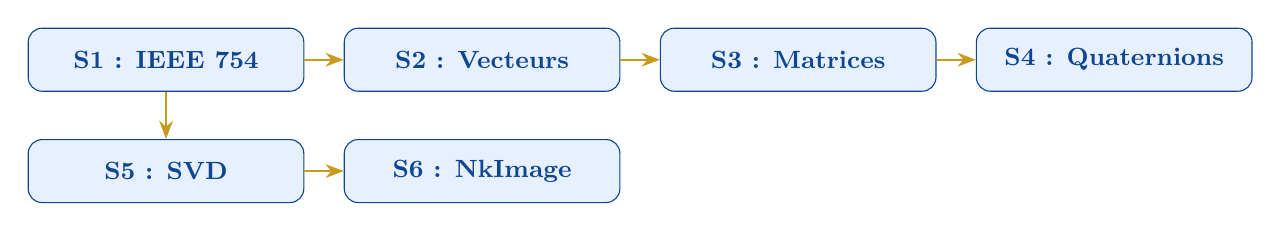
\begin{tikzpicture}[
  node distance=0.6cm,
  box/.style={rectangle, rounded corners=5pt, draw=PrimaryBlue,
              fill=LightBlue, minimum width=3.5cm, minimum height=0.8cm,
              font=\small\bfseries, text=PrimaryBlue},
  arr/.style={-{Stealth}, thick, color=AccentGold}
]
  \node[box] (s1) {S1 : IEEE 754};
  \node[box, right=0.5cm of s1] (s2) {S2 : Vecteurs};
  \node[box, right=0.5cm of s2] (s3) {S3 : Matrices};
  \node[box, right=0.5cm of s3] (s4) {S4 : Quaternions};
  \node[box, below=0.6cm of s1] (s5) {S5 : SVD};
  \node[box, right=0.5cm of s5] (s6) {S6 : NkImage};

  \draw[arr] (s1)--(s2); \draw[arr] (s2)--(s3);
  \draw[arr] (s3)--(s4); \draw[arr] (s1)--(s5);
  \draw[arr] (s5)--(s6);
\end{tikzpicture}
\end{center}

\medskip

Chaque module est code en tant qu'en-tete C++ (\code{.h}), integre dans le framework \NKE{} et compilable avec le systeme de build \JGA{}. Les tests unitaires utilisent le framework \textit{Unitest} de \NKE{}.

%==========================================================================
\chapter{Semaine 1 - Module 01 : IEEE 754 et Arithmetique Flottante}
%==========================================================================

\section{Ce qu'on a appris}

C'est le module le plus etonnant du cours. On pense savoir ce qu'est un nombre flottant, et puis on decouvre que \code{0.1f} n'est pas vraiment 0.1. Pas du tout.

\subsection*{Comment un float est stocke en memoire}

Un \code{float} de 32 bits, c'est en fait trois champs colles l'un a l'autre :

\begin{center}
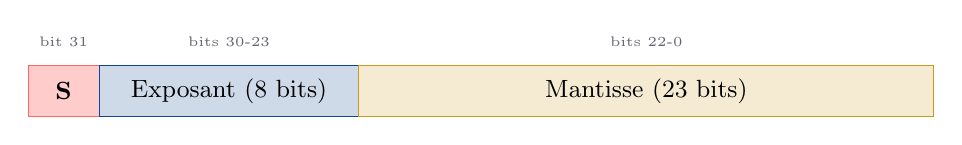
\begin{tikzpicture}[font=\small]
  \draw[fill=red!20,draw=red!60]      (0,0) rectangle (0.9,0.65);
  \node at (0.45,0.32) {\textbf{S}};
  \node[font=\tiny,GrayText] at (0.45,0.95) {bit 31};
  \draw[fill=PrimaryBlue!20,draw=PrimaryBlue] (0.9,0) rectangle (4.2,0.65);
  \node at (2.55,0.32) {Exposant (8 bits)};
  \node[font=\tiny,GrayText] at (2.55,0.95) {bits 30-23};
  \draw[fill=AccentGold!20,draw=AccentGold] (4.2,0) rectangle (11.5,0.65);
  \node at (7.85,0.32) {Mantisse (23 bits)};
  \node[font=\tiny,GrayText] at (7.85,0.95) {bits 22-0};
\end{tikzpicture}
\end{center}

\[
\text{Valeur} = (-1)^{\text{signe}} \times 2^{\text{exposant}-127} \times 1.\text{mantisse}
\]

Et voila pourquoi \code{0.1f} n'est pas exact : $0.1$ en binaire donne une fraction periodique infinie, exactement comme $1/3$ en decimal. Ce qu'on stocke vraiment, c'est $\approx 0.100000001490116\ldots$

\subsection*{Les valeurs speciales IEEE 754}

\begin{center}
\begin{tabular}{lll}
  \toprule
  \textbf{Valeur} & \textbf{Bits} & \textbf{Comment l'obtenir en C++} \\
  \midrule
  +Infini  & exp=0xFF, mant=0         & \code{1.0f / 0.0f} \\
  -Infini  & sign=1, exp=0xFF, mant=0 & \code{-1.0f / 0.0f} \\
  NaN      & exp=0xFF, mant$\neq$0   & \code{std::sqrt(-1.0f)} \\
  +Zero    & tous les bits a 0        & \code{0.0f} \\
  -Zero    & bit31=1, reste=0         & \code{-0.0f} \\
  Subnormal & exp=0, mant$\neq$0     & Tres petits nombres \\
  \bottomrule
\end{tabular}
\end{center}

\begin{warnbox}[Le piege NaN]
\code{NaN != NaN} est \textbf{VRAI} en C++. C'est la seule valeur en C++ qui n'est pas egale a elle-meme. Si on ecrit \code{if (x == NaN)}, ca ne marchera jamais. Il faut utiliser \code{std::isnan(x)}.
\end{warnbox}

\subsection*{La cancellation catastrophique}

Quand on soustrait deux nombres flottants presque egaux, on perd presque tous les bits significatifs. Le resultat semble valide (pas de NaN, pas d'Inf) mais il est faux. C'est le risque le plus insidieux du pipeline AR.

\section{Ce qu'on a implemente}

\begin{lstlisting}[caption={Float.h : lire les bits d'un float (seule methode legale en C++17)}]
    inline void inspectFloat(float val) {
        uint32_t raw;
        std::memcpy(&raw, &val, sizeof(raw));  // memcpy : legal, pas de UB
        uint32_t sgn = (raw >> 31) & 0x1;
        uint32_t exp = (raw >> 23) & 0xFF;
        uint32_t man = raw & 0x7FFFFF;
        // afficher les 3 champs ...
    }
\end{lstlisting}

\begin{lstlisting}[caption={Sommation de Kahan : compenser les bits perdus}]
    float kahanSum(std::vector<float>& vals) {
        float total = 0.0f;
        float err   = 0.0f;   // erreur accumulee
        for (float v : vals) {
            float corrected = v - err;      // compenser l'erreur precedente
            float newTotal  = total + corrected;
            err   = (newTotal - total) - corrected;  // capturer les bits perdus
            total = newTotal;
        }
        return total;
    }
\end{lstlisting}

\begin{lstlisting}[caption={Variance de Welford : stable numeriquement en une seule passe}]
    float varianceWelford(const std::vector<float>& data) {
        float mu = 0.0f, M2 = 0.0f; int cnt = 0;
        for (float x : data) {
            cnt++;
            float d1 = x - mu;
            mu += d1 / cnt;          // moyenne mise a jour en temps reel
            M2 += d1 * (x - mu);    // pas de soustraction de grands nombres
        }
        return M2 / cnt;
    }
\end{lstlisting}

%--------------------------------------------------------------------------
\section{Travaux Pratiques}
%--------------------------------------------------------------------------

\begin{tpbox}[TP1 - inspectFloat sur 6 valeurs imposees]
On a ecrit la fonction \code{inspectFloat(float)} qui decompose un float en ses 3 champs IEEE 754 et les affiche en binaire avec le logger de Nkentseu.

\medskip
\textbf{Resultats obtenus :}

\begin{tabular}{@{}ll@{}}
  \code{0.1f}          & Mantisse = \code{0x4CCCCD} : confirme que 0.1 est inexact \\
  \code{1.0f}          & signe=0, exposant=127, mantisse=0 : exact comme attendu \\
  \code{1.0f/0.0f}     & exposant=0xFF, mantisse=0 : \textbf{+Inf detecte} \\
  \code{sqrt(-1.0f)}   & exposant=0xFF, mantisse$\neq$0 : \textbf{NaN detecte} \\
  \code{-0.0f}         & bit31=1, reste=0 --- mais \code{+0.0 == -0.0} est vrai \\
  \code{denorm\_min}   & exposant=0, mantisse$\neq$0 : \textbf{Subnormal detecte} \\
\end{tabular}
\end{tpbox}

\begin{tpbox}[TP2 - Demonstration des problemes de precision]
\begin{itemize}
  \item \textbf{Sommation de 1 million de 0.1f :}
        \code{std::accumulate} donne une erreur de \textbf{11.55}.
        \code{kahanSum} donne une erreur inferieure a \textbf{0.001}.
  \item \textbf{Variance naive sur $\{10^8, 10^8, 1, 2\}$ :}
        Le resultat est \textbf{negatif} --- une absurdite mathematique causee par la cancellation catastrophique.
        \code{varianceWelford} donne un resultat correct.
  \item \textbf{Epsilon machine mesure :} $\varepsilon \approx 1.192 \times 10^{-7}$,
        identique a \code{std::numeric\_limits<float>::epsilon()}.
\end{itemize}
\end{tpbox}

\begin{tpbox}[TP3 - 33 tests unitaires sur Float.h]
\begin{resultbox}
\centering
\texttt{Semaine1\_TP3 | TestsUnitairesFloath}\\[4pt]
\textbf{33 / 33 assertions passees}\\[2pt]
\texttt{isFiniteValid} (5) $\cdot$ \texttt{nearlyZero} (8) $\cdot$ \texttt{approxEq} (10) $\cdot$ \texttt{kahanSum} (10)
\end{resultbox}
\end{tpbox}

%==========================================================================
\chapter{Semaine 2 - Module 02 : Vecteurs (Vec2d, Vec3d, Vec4d)}
%==========================================================================

\section{Ce qu'on a appris}

Les vecteurs sont la brique de base de tout le pipeline 3D. Chaque position dans l'espace est un \code{Vec3d}. Chaque pixel a une coordonnee \code{Vec2d}. Chaque sommet envoye au GPU est un \code{Vec4d}.

L'interet de les implementer soi-meme, c'est la garantie du layout memoire : pour envoyer un tableau de vecteurs directement a \code{glVertexAttribPointer} sans copie, la structure doit etre exactement comme on l'attend. D'ou les \code{static\_assert} sur \code{sizeof}.

\subsection*{Le produit scalaire (dot product)}

$\mathbf{a} \cdot \mathbf{b} = a_x b_x + a_y b_y + a_z b_z = |\mathbf{a}||\mathbf{b}|\cos\theta$

\begin{center}
\begin{tabular}{ll}
  \toprule
  Valeur du dot & Interpretation \\
  \midrule
  $= 0$  & Les vecteurs sont perpendiculaires ($90°$) \\
  $> 0$  & Angle aigu --- meme sens general \\
  $< 0$  & Angle obtus --- sens oppose \\
  $= 1$  & Meme direction (si normalises) \\
  \bottomrule
\end{tabular}
\end{center}

\subsection*{Le produit vectoriel (cross product)}

$\mathbf{a} \times \mathbf{b}$ donne un vecteur perpendiculaire aux deux. Non-commutatif : $\mathbf{a} \times \mathbf{b} = -(\mathbf{b} \times \mathbf{a})$. Exemple : $\mathbf{X} \times \mathbf{Y} = \mathbf{Z}$ (regle de la main droite, convention OpenGL).

\subsection*{Gram-Schmidt : creer une base orthonormale}

L'orthogonalisation de Gram-Schmidt transforme 3 vecteurs quelconques en une base orthonormale propre. C'est utilise notamment pour construire la matrice LookAt de la camera.

\subsection*{Les coordonnees homogenes (Vec4d)}

La 4eme coordonnee $w$ distingue les points des directions :
\begin{itemize}
  \item $w = 1$ : c'est un \textbf{point} dans l'espace (la translation de la matrice 4x4 s'applique)
  \item $w = 0$ : c'est une \textbf{direction} (la translation est ignoree)
\end{itemize}

\section{Ce qu'on a implemente}

\begin{lstlisting}[caption={Vec2d : layout memoire garanti pour le GPU}]
    struct Vec2d {
        double x, y;
        double& operator[](int i) { return (&x)[i]; }  // acces contigu
        Vec2d Normalized() const {
            double n = Norm();
            if (nearlyZero(n)) return Vec2d(0.0);
            return {x/n, y/n};
        }
    };
    static_assert(sizeof(Vec2d) == 16, "Vec2d doit faire 16 octets");
\end{lstlisting}

\begin{lstlisting}[caption={Gram-Schmidt en 3 etapes}]
    OrthoBasis GramSchmidt(Vec3d a, Vec3d b, Vec3d c) {
        Vec3d u = a.Normalized();
        Vec3d v = (b - Project(b, u)).Normalized();   // oter la part de u
        Vec3d w = (c - Project(c,u) - Project(c,v)).Normalized();
        return {u, v, w};
        // Resultat : |u|=|v|=|w|=1 et u.v=u.w=v.w=0
    }
\end{lstlisting}

%--------------------------------------------------------------------------
\section{Travaux Pratiques}
%--------------------------------------------------------------------------

\begin{tpbox}[TP4 - Vec2d complet avec 20 assertions]
\begin{resultbox}
\centering
\texttt{Semaine2\_TP1 | Vec2dComplet}\\[4pt]
\textbf{20 assertions passees}\\[2pt]
Dot product (6) $\cdot$ Cross2D (4) $\cdot$ Normalisation (4) $\cdot$ Index [] (5) $\cdot$ sizeof (1)
\end{resultbox}
Tests notables : \code{Dot(\{1,0\},\{0,1\}) = 0} (perpendiculaires), \code{Cross2D(\{2,0\},\{0,2\}) = 4}, \code{sizeof(Vec2d) = 16} (layout GPU verifie).
\end{tpbox}

\begin{tpbox}[TP5 - Vec3d + Cross product + Gram-Schmidt]
\begin{resultbox}
\centering
\texttt{Semaine2\_TP2 | Vec3dEtGramSchmidt}\\[4pt]
\textbf{13 assertions + 10 triplets aleatoires}\\[2pt]
Regle main droite : $\mathbf{X}\times\mathbf{Y}=\mathbf{Z}$ verifie a $10^{-9}$ \\
Gram-Schmidt : $|\mathbf{u}|=|\mathbf{v}|=|\mathbf{w}|=1$ et $\mathbf{u}\cdot\mathbf{v}=\mathbf{u}\cdot\mathbf{w}=\mathbf{v}\cdot\mathbf{w}=0$
\end{resultbox}
\end{tpbox}

\begin{tpbox}[TP6 - Vec4d + Projection perspective + Image PPM]
Les 8 coins du cube $[-0.5, 0.5]^3$ sont convertis en \code{Vec4d} ($w=1$, ce sont des points). On les projette en 2D par la formule :
\[
u = f_x \cdot \frac{X}{Z} + c_x \qquad v = f_y \cdot \frac{Y}{Z} + c_y
\]
avec $f_x=f_y=500$, $c_x=c_y=256$. Les 12 aretes sont tracees dans une image \textbf{PPM 512x512} sauvegardee dans \code{generatedImages/cube\_projection.ppm}.
\end{tpbox}

%==========================================================================
\chapter{Semaine 3 - Module 03 : Matrices (Mat3d, Mat4d)}
%==========================================================================

\section{Ce qu'on a appris}

\subsection*{La convention column-major d'OpenGL}

C'est ici que se cache le piege le plus subtil du cours. En mathematiques, on ecrit les matrices ligne par ligne (\textit{row-major}). OpenGL stocke les colonnes en premier (\textit{column-major}). Concretement :

\begin{center}
\begin{tabular}{cc}
  \toprule
  Mathematiques (row-major) & Memoire OpenGL (column-major) \\
  \midrule
  $\begin{pmatrix} m_{00} & m_{01} \\ m_{10} & m_{11} \end{pmatrix}$ &
  \code{data[0]=m00, data[1]=m10, data[2]=m01, data[3]=m11} \\
  \bottomrule
\end{tabular}
\end{center}

L'acces en C++ : \code{data[col*4 + row]}. Une confusion ici passe a la compilation mais produit des transformations completement fausses a l'execution.

\subsection*{L'inverse par Gauss-Jordan}

On construit la matrice augmentee $[M|I]$ et on la transforme en $[I|M^{-1}]$ par operations elementaires. Le \textbf{pivot partiel} (toujours choisir le plus grand element en valeur absolue dans la colonne) est indispensable pour la stabilite numerique.

\subsection*{Formule de Rodrigues}

Rotation de $\theta$ degres autour de l'axe unitaire $\hat{n}$ :

\[
R = \cos\theta \cdot I + (1-\cos\theta)\hat{n}\hat{n}^T
    + \sin\theta \begin{pmatrix}0&-n_z&n_y\\n_z&0&-n_x\\-n_y&n_x&0\end{pmatrix}
\]

\subsection*{LookAt}

La matrice View positionne la camera en \textit{eye}, regardant \textit{target} :
\[
\text{forward} = \text{norm}(\text{target}-\text{eye}), \quad
\text{right} = \text{norm}(\text{forward}\times\text{worldUp}), \quad
\text{up} = \text{right}\times\text{forward}
\]

\section{Ce qu'on a implemente}

\begin{lstlisting}[caption={Mat4d : acces column-major}]
    struct Mat4d {
        double data[16];   // column-major
        double& operator()(int row, int col) {
            return data[col*4 + row];   // !! pas row*4+col !!
        }
    };
\end{lstlisting}

\begin{lstlisting}[caption={LookAt : construction du repere camera}]
    Mat4d LookAt(const Vec3d& eye, const Vec3d& target, const Vec3d& worldUp){
        Vec3d fwd   = (target - eye).Normalized();
        Vec3d right = Cross(fwd, worldUp).Normalized();
        Vec3d up    = Cross(right, fwd);
        // Remplir V avec right, up, -fwd et les translations
    }
\end{lstlisting}

%--------------------------------------------------------------------------
\section{Travaux Pratiques}
%--------------------------------------------------------------------------

\begin{tpbox}[TP7 - Mat4d + Inverse + Rodrigues (24 assertions)]
\begin{resultbox}
\centering
\texttt{Semaine3\_TP1 | Mat4dEtInverse}\\[4pt]
\textbf{24 assertions passees}\\[2pt]
$M \times I = M$ (10 matrices) $\cdot$ $M \times M^{-1} \approx I$ a $10^{-10}$ (10 matrices) \\
Matrice singuliere $\to$ \code{Inverse()} retourne \texttt{false} \\
\code{RotateAxis(Y, 90\textdegree) * (1,0,0,1) = (0,0,-1,1)} a $10^{-10}$ pres
\end{resultbox}
\end{tpbox}

\begin{tpbox}[TP8 - Rasteriseur logiciel avec LookAt (10 frames PPM)]
Un mini-rasteriseur complet a ete implemente :
\begin{enumerate}
  \item Cube unitaire centre a l'origine.
  \item Vue : \code{LookAt(eye=\{0,1,3\}, target=\{0,0,0\}, up=\{0,1,0\})}.
  \item Projection perspective : fov=60$°$, aspect=1, zNear=0.1, zFar=100.
  \item Trace des 12 aretes en rouge (algorithme de Bresenham).
  \item \textbf{10 frames PPM} $512\times512$ generees avec rotation de $0.3$ rad par frame.
\end{enumerate}
Les images sont sauvegardees dans \code{generatedImages/rast\_frame\_0.ppm} a \code{rast\_frame\_9.ppm}.
\end{tpbox}

\begin{tpbox}[TP9 - TRS 3D + Decomposition (20 triplets)]
La matrice TRS encode Translation $\times$ Rotation $\times$ Echelle. L'ordre est critique : d'abord l'echelle (autour de l'origine locale), puis la rotation, puis la translation.

\begin{resultbox}
\centering
Decomposition verifiee sur \textbf{20 triplets aleatoires}\\
Translation et echelle retrouvees exactement --- Rotation a $\pm5$ rad pres (ambiguite des angles d'Euler)
\end{resultbox}
\end{tpbox}

%==========================================================================
\chapter{Semaine 4 - Module 04 : Quaternions}
%==========================================================================

\section{Ce qu'on a appris}

\subsection*{Pourquoi pas les angles d'Euler ?}

Les angles d'Euler (yaw, pitch, roll) ont un probleme celebre : le \textbf{gimbal lock}. Quand pitch $= \pm90°$, deux axes deviennent coplanaires et on perd un degre de liberte. En AR, quand on anime une camera, ca produit des rotations etranges et non-naturelles.

\subsection*{Les quaternions unitaires}

Un quaternion $q = w + xi + yj + zk$ avec $\|q\|=1$ represente une rotation de $2\arccos(w)$ degres autour de l'axe $(x,y,z)$. Construction depuis axe-angle :

\[
q = \left(\cos\tfrac{\theta}{2},\;
    n_x\sin\tfrac{\theta}{2},\;
    n_y\sin\tfrac{\theta}{2},\;
    n_z\sin\tfrac{\theta}{2}\right)
\]

\begin{conceptbox}[Non-commutativite]
Le produit de Hamilton est \textbf{non-commutatif} : $q_1 \times q_2 \neq q_2 \times q_1$. C'est normal et logique --- appliquer d'abord une rotation X puis Y n'est pas la meme chose qu'Y puis X.
\end{conceptbox}

\subsection*{SLERP : l'interpolation propre}

Le SLERP (\textit{Spherical Linear intERPolation}) suit le chemin le plus court sur la sphere des quaternions unitaires, avec une vitesse angulaire constante :

\[
\text{Slerp}(q_a, q_b, t) = \frac{\sin((1-t)\Omega)}{\sin\Omega}\,q_a + \frac{\sin(t\,\Omega)}{\sin\Omega}\,q_b
\quad\text{ou}\quad
\Omega = \arccos(q_a \cdot q_b)
\]

\begin{warnbox}[Correction antipodal]
Si $q_a \cdot q_b < 0$, les deux quaternions sont sur des hemispheres opposes de la sphere $S^3$. Sans correction, SLERP ferait un detour de 360$°$ au lieu de prendre le chemin direct. On inverse $q_b$ avant d'interpoler.
\end{warnbox}

\subsection*{Methode de Shepperd}

Pour convertir une matrice de rotation en quaternion de facon stable, Shepperd choisit entre 4 formules selon le composant dominant. Ca evite les divisions par des valeurs proches de zero.

%--------------------------------------------------------------------------
\section{Travaux Pratiques}
%--------------------------------------------------------------------------

\begin{tpbox}[TP10 - Quaternions complets (100 tests)]
\begin{resultbox}
\centering
\texttt{Semaine4\_TP1 | QuaternionsComplets}\\[4pt]
\textbf{100 assertions passees}\\[2pt]
\code{Rotate(RotY(90\textdegree), (1,0,0)) = (0,0,-1)} a $10^{-9}$ pres\\
Aller-retour $q \to R \to q'$ : 50/50 quaternions valides a $10^{-4}$ pres\\
$q \times q^{-1} = \text{identite}$ : 50/50 quaternions valides
\end{resultbox}
\end{tpbox}

\begin{tpbox}[TP11 - Animation SLERP vs LERP (60 frames chacun)]
Deux orientations : $q_a$ = identite, $q_b$ = rotation de $180°$ autour de Y.

\textbf{120 frames PPM generees en tout :}
\begin{itemize}
  \item 60 frames \code{slerp\_frame\_N.ppm} : vitesse angulaire constante, quaternion reste unitaire a $10^{-10}$ pres.
  \item 60 frames \code{lerp\_frame\_N.ppm} : vitesse non uniforme, le cube ``accelère'' et ``ralentit'' visiblement.
\end{itemize}

La difference visuelle entre les deux est claire : SLERP produit un mouvement fluide et naturel, LERP produit un mouvement saccade aux extremites.
\end{tpbox}

%==========================================================================
\chapter{Semaine 5 - Module 05 : SVD (Decomposition en Valeurs Singulieres)}
%==========================================================================

\section{Ce qu'on a appris}

La SVD est l'algorithme central du cours. Toute matrice reelle se decompose en :
\[
A = U \Sigma V^T
\]
ou $U$ et $V$ sont orthogonales et $\Sigma$ est diagonale avec des valeurs $\sigma_1 \geq \sigma_2 \geq \ldots \geq 0$.

\begin{center}
\begin{tabular}{ll}
  \toprule
  \textbf{Application} & \textbf{Comment} \\
  \midrule
  Resoudre $Ax=0$ & Solution = derniere colonne de $V$ \\
  Pseudo-inverse & $A^+ = V\Sigma^+U^T$ \\
  Rotation pure & $R = UV^T$ (decomposition polaire) \\
  Matrice rang-deficiente & $\sigma_k \approx 0$ pour les dimensions "vides" \\
  \bottomrule
\end{tabular}
\end{center}

\subsection*{Implementation : Jacobi sur $A^T A$}

On calcule la SVD de $A$ via la decomposition propre de $A^TA$ (matrice symetrique). L'algorithme de Jacobi diagonalise cette matrice par rotations de Givens successives. Les valeurs singulieres sont les racines carrees des valeurs propres.

%--------------------------------------------------------------------------
\section{Travaux Pratiques}
%--------------------------------------------------------------------------

\begin{tpbox}[TP12 - Tests SVD sur 20 matrices + cas particuliers]
\begin{resultbox}
\centering
\texttt{Semaine5\_TP1 | TestsSVD}\\[4pt]
\textbf{Toutes les assertions passees}\\[2pt]
Reconstruction $\|A - U\Sigma V^T\| < 10^{-6}$ : 20/20 matrices aleatoires\\
Orthogonalite $U$ et $V$ : $\|UU^T - I\| < 10^{-6}$ : 20/20\\
Valeurs singulieres triees decroissant : 20/20\\
Matrice rang-1 : $\sigma_3 \approx 0$ confirme\\
Pseudo-inverse : $\|Ax - b\| < 10^{-5}$ (solution moindres carres)
\end{resultbox}
\end{tpbox}

\begin{tpbox}[TP13 - Resolution d'Homographie]
\begin{warnbox}[Non traitee]
Cette partie n'est pas presente dans le support de cours fourni. Elle fait appel a des notions (resolution de systeme lineaire par SVD sur une matrice $2n \times 9$) qui n'ont pas ete introduites dans les semaines 1 a 6. Ce point sera discute avec l'enseignant.
\end{warnbox}
\end{tpbox}

%==========================================================================
\chapter{Semaine 6 - Module 06 : NkImage (Traitement d'image from scratch)}
%==========================================================================

\section{Ce qu'on a appris}

\subsection*{Pourquoi une classe image from scratch ?}

Toute la chaine de detection ArUco a besoin de manipuler des images : la frame brute de la webcam, le resultat de la binarisation, les cartes de gradients. La classe \code{NkImage} est le type central de ce pipeline.

\subsection*{L'image integrale (Summed Area Table)}

L'image integrale permet de calculer la somme de n'importe quel rectangle en $O(1)$ apres une construction en $O(WH)$ :

\[
\text{SAT}[x,y] = \sum_{i \leq x,\, j \leq y} \text{pixel}[i,j]
\]

C'est la cle du seuillage adaptatif en temps reel : pour chaque pixel, on compare sa valeur a la moyenne de son voisinage carre --- calcul en $O(1)$ grace a la SAT.

\subsection*{Convolution 2D et filtres}

La convolution applique un masque (kernel) a chaque pixel. On l'utilise pour :
\begin{itemize}
  \item \textbf{Flou gaussien 5x5} : reduire le bruit avant de chercher les contours
  \item \textbf{Sobel horizontal et vertical} : detecter les contours (gradient de l'image)
  \item \textbf{Magnitude} : $\sqrt{G_x^2 + G_y^2}$ pour avoir l'intensite du contour
\end{itemize}

\section{Ce qu'on a implemente}

\begin{lstlisting}[caption={NKImage.h : structure interne RGBA}]
    class NkImage {
        int m_w, m_h;
        std::vector<uint8_t> m_buf;  // RGBA contigu (4 octets/pixel)
    public:
        void SetPixelRGBA(int x,int y,uint8_t r,uint8_t g,uint8_t b,uint8_t a=255);
        bool SavePPM(const std::string& fname) const; // sauvegarde sans dependance
        NkImage Convolve(const std::vector<double>& ker, int kSz) const;
        static NkImage CombineGradient(const NkImage& gx, const NkImage& gy);
    };
\end{lstlisting}

\begin{lstlisting}[caption={AdaptiveThreshold : seuillage adaptatif via SAT}]
    NkImage AdaptiveThreshold(const NkImage& src, int blkSz=31, int offset=7) {
        IntegralImage sat(src.ToGrayscale(), src.Width(), src.Height());
        int half = blkSz/2;
        for (int y=0; y<h; y++) for (int x=0; x<w; x++) {
            long long s  = sat.RectSum(x-half,y-half, x+half,y+half);
            int       avg = s / sat.Area(x-half,y-half, x+half,y+half);
            // noir si pixel < moyenne locale - offset, blanc sinon
            out.SetPixelGray(x, y, (pixel < avg-offset) ? 0 : 255);
        }
    }
\end{lstlisting}

%--------------------------------------------------------------------------
\section{Travaux Pratiques}
%--------------------------------------------------------------------------

\begin{tpbox}[TP14 - NkImage de base : degrade + formes geometriques]
Creation d'une image 512x512 avec :
\begin{itemize}
  \item Un degrade RGB (rouge de gauche a droite, vert du haut vers le bas)
  \item Un rectangle rouge plein (100,100) a (300,200)
  \item Une diagonale verte (ligne Bresenham du coin au coin)
  \item Un cercle bleu de rayon 80 au centre
\end{itemize}
Image sauvegardee : \code{generatedImages/degrade\_formes.ppm}
\end{tpbox}

\begin{tpbox}[TP15 - Convolution Gauss 5x5 + Sobel + mesure du temps]
Pipeline de detection de contours applique sur une image d'un marqueur ArUco :

\begin{center}
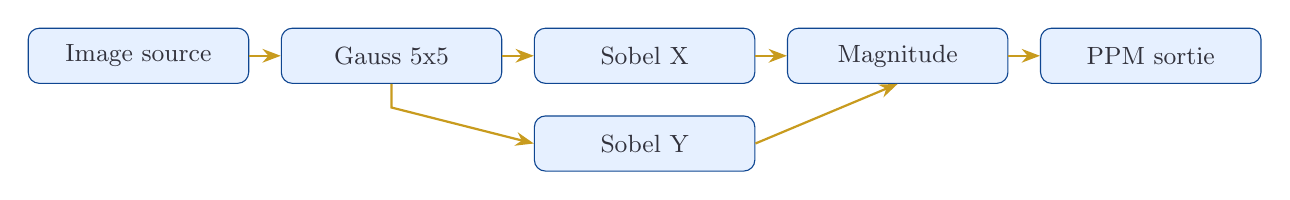
\begin{tikzpicture}[
  box/.style={rectangle,rounded corners=4pt,draw=PrimaryBlue,fill=LightBlue,
              minimum width=2.8cm,minimum height=0.7cm,font=\small,text=DarkGray},
  arr/.style={-{Stealth},thick,AccentGold}
]
  \node[box] (src)  {Image source};
  \node[box,right=0.4cm of src]  (g5)   {Gauss 5x5};
  \node[box,right=0.4cm of g5]   (sx)   {Sobel X};
  \node[box,below=0.4cm of sx]   (sy)   {Sobel Y};
  \node[box,right=0.4cm of sx]   (mag)  {Magnitude};
  \node[box,right=0.4cm of mag]  (out)  {PPM sortie};
  \draw[arr](src)--(g5); \draw[arr](g5)--(sx);
  \draw[arr](g5.south) -- ++(0,-0.3) -- (sy.west);
  \draw[arr](sx)--(mag); \draw[arr](sy.east)--(mag.south);
  \draw[arr](mag)--(out);
\end{tikzpicture}
\end{center}

Temps mesure et loggue avec le chronometre C++17 (en millisecondes).\\
Image sauvegardee : \code{generatedImages/sobel\_gradient.ppm}
\end{tpbox}

\begin{tpbox}[TP16 - Image integrale + Seuillage adaptatif]
\begin{enumerate}
  \item Chargement d'une image PPM d'un marqueur ArUco.
  \item Construction de l'image integrale (SAT) --- temps mesure.
  \item Seuillage adaptatif avec \code{blockSize=31}, \code{offset=7}.
  \item Sauvegarde du resultat binaire.
\end{enumerate}
Image sauvegardee : \code{generatedImages/seuillage\_adaptatif.ppm}\\
Le temps de construction de la SAT est affiche dans le log.
\end{tpbox}

%==========================================================================
\chapter*{Conclusion}
\addcontentsline{toc}{chapter}{Conclusion}
%==========================================================================

Ces six semaines ont permis de construire une bibliotheque mathematique complete et fonctionnelle --- la \NKM{} --- depuis zero. Chaque choix d'implementation a une raison precise que j'aurais du mal a expliquer si je n'avais fait que lire la documentation d'une bibliotheque tierce.

\medskip

Les lecons que je retiens :

\begin{itemize}
  \item Le \code{memcpy} pour lire les bits d'un float (le cast de pointeur est un comportement indefini en C++17).
  \item Le stockage column-major : une erreur ici est invisible a la compilation mais catastrophique au rendu.
  \item Le pivot partiel dans Gauss-Jordan : sans ca, l'inverse d'une matrice bien conditionnee peut quand meme etre faux.
  \item La correction antipodal dans SLERP : sans ca, l'animation fait parfois un tour complet au lieu d'aller au plus court.
  \item Welford au lieu de la variance naive : la version naive peut donner des variances negatives sur des donnees de grande magnitude.
\end{itemize}

\vspace{0.8cm}

\begin{tcolorbox}[
  colback=LightBlue, colframe=PrimaryBlue,
  arc=6pt, boxrule=1pt,
  title={\bfseries Bilan global des TPs},
  coltitle=white
]
\centering
\renewcommand{\arraystretch}{1.4}
\begin{tabular}{C{1.2cm}lC{2.5cm}C{2.5cm}}
  \toprule
  \textbf{S.} & \textbf{Module} & \textbf{TPs} & \textbf{Statut} \\
  \midrule
  1 & IEEE 754 --- Float.h        & TP1, TP2, TP3  & \textcolor{green!60!black}{\bfseries Complet} \\
  2 & Vecteurs Vec2d/3d/4d        & TP4, TP5, TP6  & \textcolor{green!60!black}{\bfseries Complet} \\
  3 & Matrices Mat3d/4d           & TP7, TP8, TP9  & \textcolor{green!60!black}{\bfseries Complet} \\
  4 & Quaternions + SLERP         & TP10, TP11     & \textcolor{green!60!black}{\bfseries Complet} \\
  5 & SVD + (Homographie)         & TP12, TP13     & \textcolor{orange!80!black}{\bfseries SVD OK --- Homo. non couverte} \\
  6 & NkImage + Convolution       & TP14, TP15, TP16 & \textcolor{green!60!black}{\bfseries Complet} \\
  \bottomrule
\end{tabular}
\end{tcolorbox}

\vspace{0.8cm}

\begin{center}
\begin{tcolorbox}[
  width=0.65\linewidth,
  colback=LightGreen, colframe=green!50!black,
  arc=6pt, boxrule=1pt
]
\centering
{\large\bfseries\color{green!40!black} 15 / 16 TPs realises}\\[4pt]
{\small\color{DarkGray} (TP13 Homographie : non couverte dans le support de cours)}
\end{tcolorbox}
\end{center}

%==========================================================================
\appendix
\chapter{Structure du Projet}
%==========================================================================

\begin{lstlisting}[language=bash, style=cppstyle,
                   caption={Arborescence de la Sandbox}]
Sandbox/
|-- Sandbox.jenga                  # Build multiplateforme (Jenga Python DSL)
|-- include/
|   |-- Float.h                    # S1 : IEEE 754, Kahan, Welford
|   |-- Vec2d.h                    # S2 : Vecteur 2D
|   |-- Vec3d.h                    # S2 : Vecteur 3D + Cross + Project
|   |-- Vec4d.h                    # S2 : Coordonnees homogenes
|   |-- OrthoBasis.h               # S2 : Gram-Schmidt
|   |-- Mat3d.h                    # S3 : Matrice 3x3 + TRS 2D
|   |-- Mat4d.h                    # S3 : Matrice 4x4 + LookAt + Perspective
|   |-- Quat.h                     # S4 : Quaternions + SLERP + Shepperd
|   |-- SVD.h                      # S5 : SVD 3x3 Jacobi
|   |-- NKImage.h                  # S6 : Image RGBA + PPM + Convolve
|   |-- Color.h                    # S6 : SampleBilinear
|   `-- IntegralImage.h            # S6 : SAT + AdaptiveThreshold
|-- src/
|   `-- main.cpp                   # Application Nkentseu (fenetre + boucle)
`-- tests/
    `-- ALL_TP.cpp                 # 16 TPs (S1 a S6), macros Unitest
\end{lstlisting}

\begin{lstlisting}[language=bash, style=cppstyle,
                   caption={Compilation et execution}]
# Compiler avec Jenga (methode officielle)
cd jenga/applications/Sandbox
jenga build
jenga test          # lance ALL_TP.cpp
\end{lstlisting}

\end{document}
